\cleartorightpage
\begin{savequote}[75mm]
“As always in life, people want a simple answer \ldots and it’s always wrong.”
\qauthor{Susan Greenfield}
\end{savequote}

\chapter{Structural Variant Analysis}\label{chapter:fusiongenes}
\setcounter{figure}{-1}
\setcounter{table}{-1}
\setcounter{section}{-1}

\begin{figure}[t!]
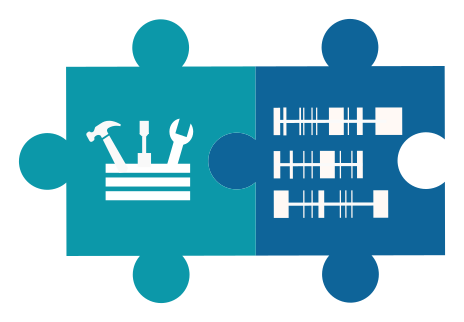
\includegraphics[height=10em]{frontmatter/images/chapter-header-fusion-tools.png}
\end{figure}
\setcounter{figure}{-1}
\setcounter{table}{-1}
\setcounter{section}{-1}


Structural variations (SVs) are large-scale rearrangements of the genome. When these alterations occur within genes, novel hybrid genes called \emph{fusion genes} may be formed. Accurate detection of these SVs and resulting fusion genes are informative for e.g. diagnostics in cancer analysis.

We created iFUSE, a web-based application to visualize and explore structural variants, and identify and prioritize potential fusion genes within a sample. We subsequently used this tool to detect multiple fusions in the VCaP cell line. Furthermore, we discovered the presence of chromothripsis on chromosome 5q of this sample, and used the Circos tool to visualize this in a single plot.

This chapter contains the following sub-chapters:

\begin{enumerate}[label=\ref{chapter:fusiongenes}.\arabic*]
\itemsep-0.5em
\setcounter{enumi}{-1}
\item \textbf{iFUSE: integrated fusion gene explorer.}
In this work, we created an interactive web-based visualisation tool for the identification and prioritization of fusion gene candidates. Coding of the application was initiated by Jos van Nijnatten (PHP web framework) and Elizabeth McClellan (R data analysis), and later finalized and further adapted by myself (PHP, R \& bash). I also worked to increase the interoperability of the code, extending it to additional file formats beyond Complete Genomics. Together with Ines Teles Alves, I worked to validate the application. Ivo Palli made sure the application was available as a robust web service to visitors from outside the EMC. However, due to changed policies at the EMC in the intervening years, we are no longer allowed to offer the iFUSE application as a service to users from outside the EMC network. Therefore, the link mentioned in this work is no longer functional. In order to keep iFUSE freely available to all, I have created a Docker image of the application, allowing anybody to run iFUSE on their own machines. Please see the GitHub repository at \url{https://github.com/erasmusmc-bioinformatics/ifuse} for further details.

\item \textbf{Gene fusions by chromothripsis of chromosome 5q in the VCaP prostate cancer cell line.}
In this work, we used the iFUSE application to identify and validate fusion gene candidates. I led the bioinformatics analysis while Ines Teles Alves led the experimental validation. While we analyzed many samples, we came across a surprise in the VCaP sample, it seemed to display chromothripsis on the q arm of chromosome 5. We were able to confirm this through a combination of bioinformatic analysis and experimental validation.


\end{enumerate}


